%%%%%%%%%%%%%%%%%%%%%%%%%%%%%%%%%%%%%%%%%
% Journal Article
% LaTeX Template
% Version 1.4 (15/5/16)
%
% This template has been downloaded from:
% http://www.LaTeXTemplates.com
%
% Original author:
% Frits Wenneker (http://www.howtotex.com) with extensive modifications by
% Vel (vel@LaTeXTemplates.com)
%
% License:
% CC BY-NC-SA 3.0 (http://creativecommons.org/licenses/by-nc-sa/3.0/)
%
%%%%%%%%%%%%%%%%%%%%%%%%%%%%%%%%%%%%%%%%%

%----------------------------------------------------------------------------------------
%	PACKAGES AND OTHER DOCUMENT CONFIGURATIONS
%----------------------------------------------------------------------------------------

\documentclass[twoside,twocolumn]{article}

\usepackage{blindtext} % Package to generate dummy text throughout this template 

\usepackage[sc]{mathpazo} % Use the Palatino font
\usepackage[T1]{fontenc} % Use 8-bit encoding that has 256 glyphs
\linespread{1.05} % Line spacing - Palatino needs more space between lines
\usepackage{microtype} % Slightly tweak font spacing for aesthetics

\usepackage[english]{babel} % Language hyphenation and typographical rules

\usepackage[hmarginratio=1:1,top=32mm,columnsep=20pt]{geometry} % Document margins
\usepackage[hang, small,labelfont=bf,up,textfont=it,up]{caption} % Custom captions under/above floats in tables or figures
\usepackage{booktabs} % Horizontal rules in tables

\usepackage{lettrine} % The lettrine is the first enlarged letter at the beginning of the text

\usepackage{enumitem} % Customized lists
\setlist[itemize]{noitemsep} % Make itemize lists more compact

\usepackage{abstract} % Allows abstract customization
\renewcommand{\abstractnamefont}{\normalfont\bfseries} % Set the "Abstract" text to bold
\renewcommand{\abstracttextfont}{\normalfont\small\itshape} % Set the abstract itself to small italic text

\usepackage{titlesec} % Allows customization of titles
\renewcommand\thesection{\Roman{section}} % Roman numerals for the sections
\renewcommand\thesubsection{\roman{subsection}} % roman numerals for subsections
\titleformat{\section}[block]{\large\scshape\centering}{\thesection.}{1em}{} % Change the look of the section titles
\titleformat{\subsection}[block]{\large}{\thesubsection.}{1em}{} % Change the look of the section titles

\usepackage{fancyhdr} % Headers and footers
\pagestyle{fancy} % All pages have headers and footers
\fancyhead{} % Blank out the default header
\fancyfoot{} % Blank out the default footer
\fancyhead[C]{System Design $\bullet$ Nov 2018} % Custom header text
\fancyfoot[RO,LE]{\thepage} % Custom footer text

\usepackage{titling} % Customizing the title section

\usepackage{hyperref} % For hyperlinks in the PDF

\usepackage{booktabs}
\usepackage{multirow}
\usepackage{framed}
\usepackage{caption}
\usepackage{graphicx}

%----------------------------------------------------------------------------------------
%	TITLE SECTION
%----------------------------------------------------------------------------------------

\setlength{\droptitle}{-4\baselineskip} % Move the title up

\pretitle{\begin{center}\Huge\bfseries} % Article title formatting
\posttitle{\end{center}} % Article title closing formatting
\title{System design report: Multi-Agent System} % Article title
\author{%
\textsc{James King} \\% Your name
\normalsize Supervisor: Kostas Stathis \\ % Your supervisor
}
\date{October 2018} % Leave empty to omit a date
\renewcommand{\maketitlehookd}{%
\begin{abstract}
Architectures and designs for intelligent agents and the environment they reside come in many different variations. For my multi-agent system I need to make some decisions to match a design for agents and their environment to the model I laid out in my report on indirect reciprocity. To do this I will consider different agent architectures, features and designs, considering how closely they match the model before laying out an architecture of my own. I shall also consider the properties of the environment the agents reside in before laying out a concrete execution for a game of indirect reciprocity. From these two component definitions I will formulate a method of communication between the environment and the agents service.
\end{abstract}
}

%----------------------------------------------------------------------------------------

\begin{document}

%Milestone: Report on the design of the Prolog service and Agents, and the web application and agent’s environment
%Will include the following: an agent definition and the inner workings of an agent’s decision-making component, a definition of the structure of the Prolog service and management of agents (as well as the design of the API), a definition of the agent’s environment and how this will work with the Prolog service, and a design of the web application. This is key to a well-planned architecture for the Prolog service and agent environment. It will also help me research better methods of implementation for the Prolog service.
% Link to goal: This will lay out a concrete way of implementing the Prolog service, web application and link between them.

% Print the title
\maketitle

%----------------------------------------------------------------------------------------
%	ARTICLE CONTENTS
%----------------------------------------------------------------------------------------

\section{Introduction}
One of the aims of my project is to produce a multi-agent system to play games of indirect reciprocity, the model for which I have defined in my second report: ``Report on indirect reciprocity, strategies for agents and the development of a concrete model to implement''. For this I have designed a system that includes two main components: The environment and a web service to host agent's decision making components (see figure~\ref{fig:syspackage}).\\
I have already decided on a web service to host agent's minds for a number of reasons. One of the reasons being that in interactions across a network agents provide an API to work with (much like the API I will be providing). Meaning that it is good practice for me to consider how an API for an agent can be designed and deployed. Another reason is the difficulty interfacing between prolog and python and finally that a key use case for agents is as part of distributed systems, so using a web service to deploy them brings me closer to a real use case.\\
In my project, I will be hosting the environment in my Flask web application, but, the aim is for the environment to be used as if it is a library, as long as it is connected to an application/service that runs agent's decision making component. As such I will not be addressing how the web application hosting the environment, but the environment itself and the agents service.
\begin{figure}
	\begin{center}
	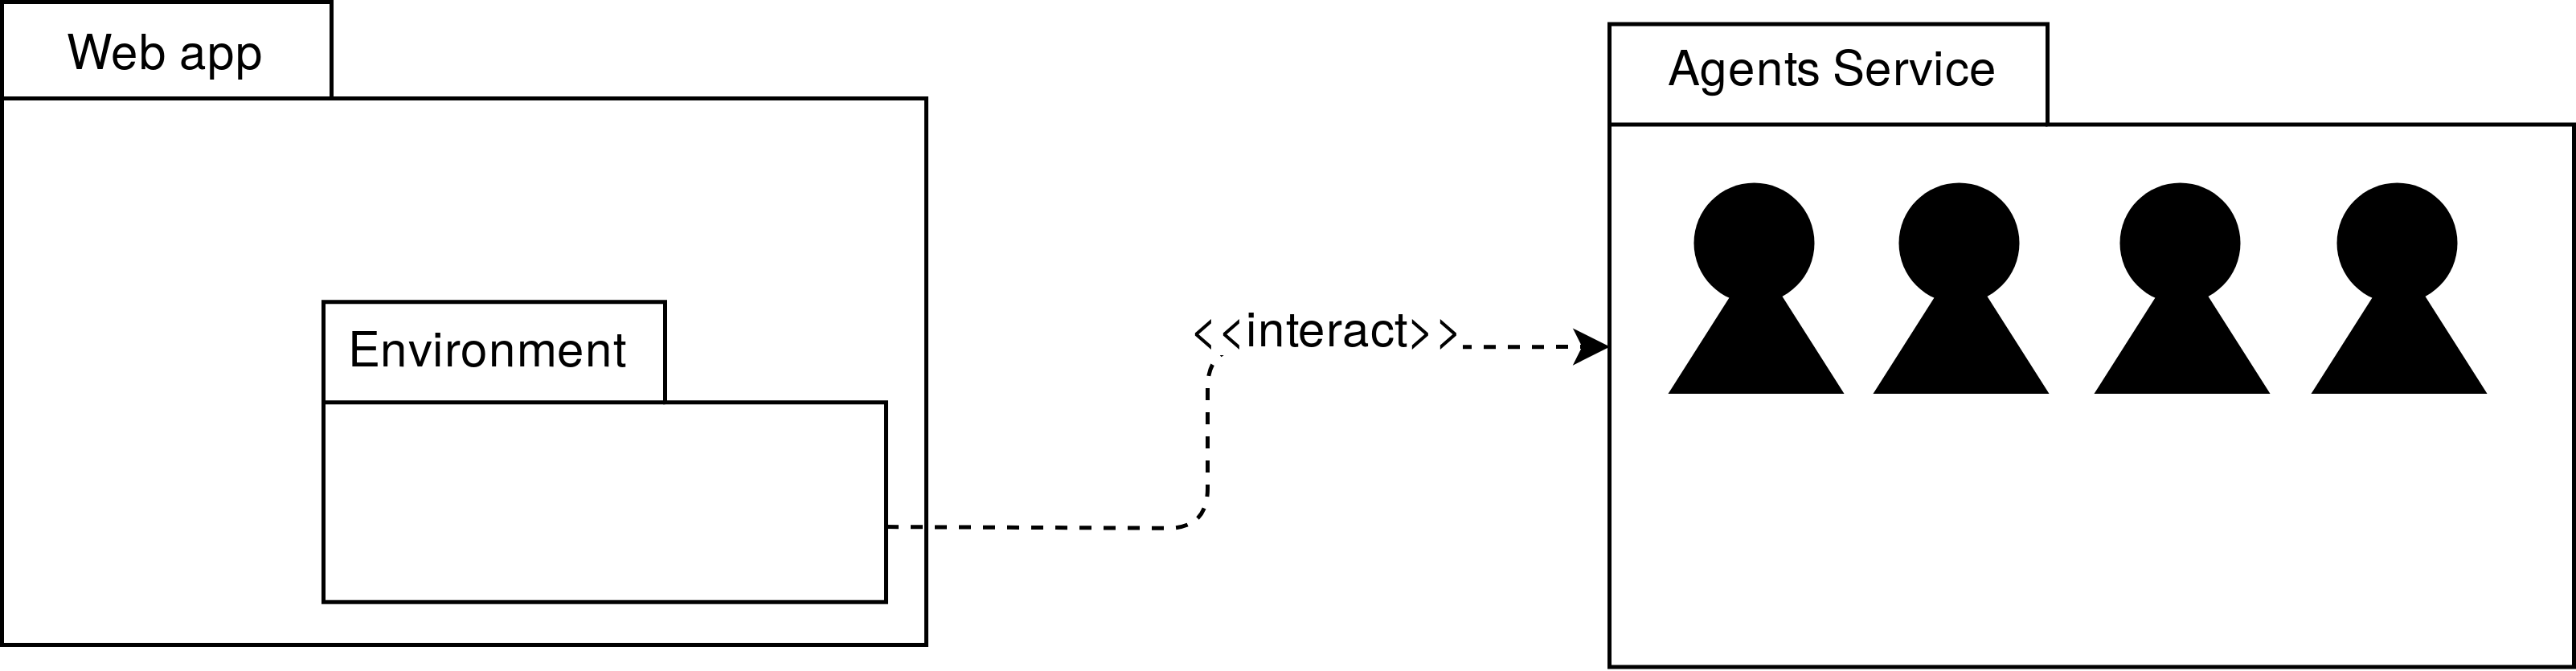
\includegraphics[width=0.5\textwidth]{SystemPackage.png}
	\caption{UML Package diagram to display the system components}
	\label{fig:syspackage}
	\end{center}
\end{figure}

%------------------------------------------------

\section{Content and Knowledge}
This section I will split up into 3 parts: one for each of the two main components - the environment and agents minds service and another for the communication between these two components.
\subsection{Agents}
There are many different definitions of what properties a system needs in order to be considered an agent. One definition containing 4 properties was proposed by Wooldridge and Jennings~\cite{wooldridge_jennings_1995}: autonomy, reactivity, proactivity and social ability.\\
Autonomy being considered the ability to operate without direct human intervention and having control over the agent's own actions and internal state. Reactivity is defined as agents perceiving their environment and responding to changes in it in a timely fashion. Proactivity is given as the ability to exhibit goal-driven behaviour, rather than just reacting to its environment. Lastly, social ability is interaction between agents and/or humans via an ACL (agent communication language).\\
This notion of using the 4 properties to define an agent is considered a `weak' notion. Wooldridge and Jennings suggest that stronger notions of agency include more human-like features. One such human-like feature that exists in game-theoretic models is the idea of memory or an internal state that the agent can act on. An internal state is used in Russell and Norvig's model-based reflex agent which takes percepts, modifies it's internal state and uses the internal state and a model of the environment as input to condition-action rules as seen in figure~\ref{fig:model_reflex}.
\begin{figure}
	\begin{center}
	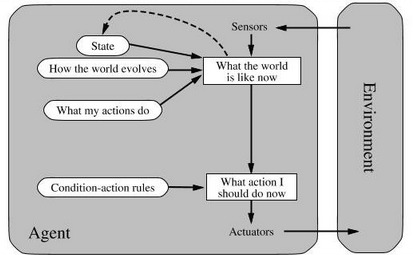
\includegraphics[width=0.5\textwidth]{RuNorv.png}
	\caption{A model-based reflex agent from Russell and Norvig~\cite{russell2016artificial}.}
	\label{fig:model_reflex}
	\end{center}
\end{figure}
\noindent The model-based reflex agent architecture can be applied as an example to a game-theoretic agent strategy known as an image scoring discriminator, as laid out by Nowak and Sigmund~\cite{evol_indirect_image}. An image scoring discriminator's condition-action rules state: if the discriminator's internal state is greater than or equal to $k$ (a variable set at the initialization of the agent) it is best to cooperate, else the agent will defect. The image scores are held in an agent's internal state and may change depending on the percepts the image scoring discriminator agent receives.\\
Some game-theoretic strategies don't use memory or internal state and just seek to provide a theory to act on. Though this does not qualify them as an agent according to Wooldridge and Jennings~\cite{wooldridge_jennings_1995} they are still relevant strategies for game-theory.\\
These indirect reciprocity strategies bear a remarkable resemblance to both model-based reflex agents and how theories are encoded in deductive reasoning agents. Deductive reasoning agents use theories to encode how it is best to act under any given situation~\cite{kostas_deductive}. Agents who follow the image score discriminator strategy could have a theory encoded in them such as:
\begin{framed}
\noindent$interaction(me, Recipient, time) \wedge image\_score(me, Recipient, Score, time) \wedge Score\geq k \to do(cooperate(Recipient))$\\\\
$interaction(me, Recipient, time) \wedge image\_score(me, Recipient, Score, time) \wedge Score<k \to do(defect(Recipient))$\\\\
$\neg interaction(me, \_, time) \to do(idle)$
\end{framed}
\noindent Part of the deductive reasoning agents method of implementing agents is the logical database that includes information on the current state of the world. In the example above this would possibly include logical data such as:
\begin{framed}
\begin{center}
$image\_score(agent1, agent2, 2, 9).$ \\
$interaction(agent1, agent2, 6).$
\end{center}
\end{framed}
\noindent This logical database is similar to the model-based reflex agent architecture's internal state and the human-like concept of belief. Beliefs as a mental category is included in the language Agent0 presented by Yoav Shoham~\cite{shoham1991agent0} as one of his two mental categories: belief and commitment.\\
He defines beliefs as a fact that is thought to be true by an agent at a specific time about a specific time (an agent is constrained to not believe contradictory facts). Commitments are given as a commitment to act (restricted by the agent's capabilities) not a commitment to pursue a goal.\\
Agent capabilities are another concept Shoham uses and are defined as relations between the agent's mental state and their environment. An agent is only capable of committing to an action iff they believe themselves to be capable. In my example above this is shown by the agent only being capable of defecting or cooperating if they are a donor in an interaction.\\
In my system, I wish to incorporate similar ideas to those I have mentioned: beliefs (internal state), commitments, capabilities and strategies (deductive reasoning theories). Russell and Norvig specify that an agent can be thought of as a system that perceives its environment and acts within it~\cite{russell2016artificial}. They then go on to explain that an agent maps percept sequences to actions. In the system I am producing, this mapping will be similar to model-based reflex agents. The mapping will be provided by changing the agent's internal state based on the percepts an agent receives and then deciding on an action to take, based on this internal state/beliefs, by way of a deductive reasoning theory.\\
Percepts in my system will include an observation of an action (either cooperating or defecting), an observation of a gossip action (either positive or negative) and perceiving that they are a member of a donor-recipient pair at a given timepoint (and which role they hold).
\begin{figure}
	\begin{center}
	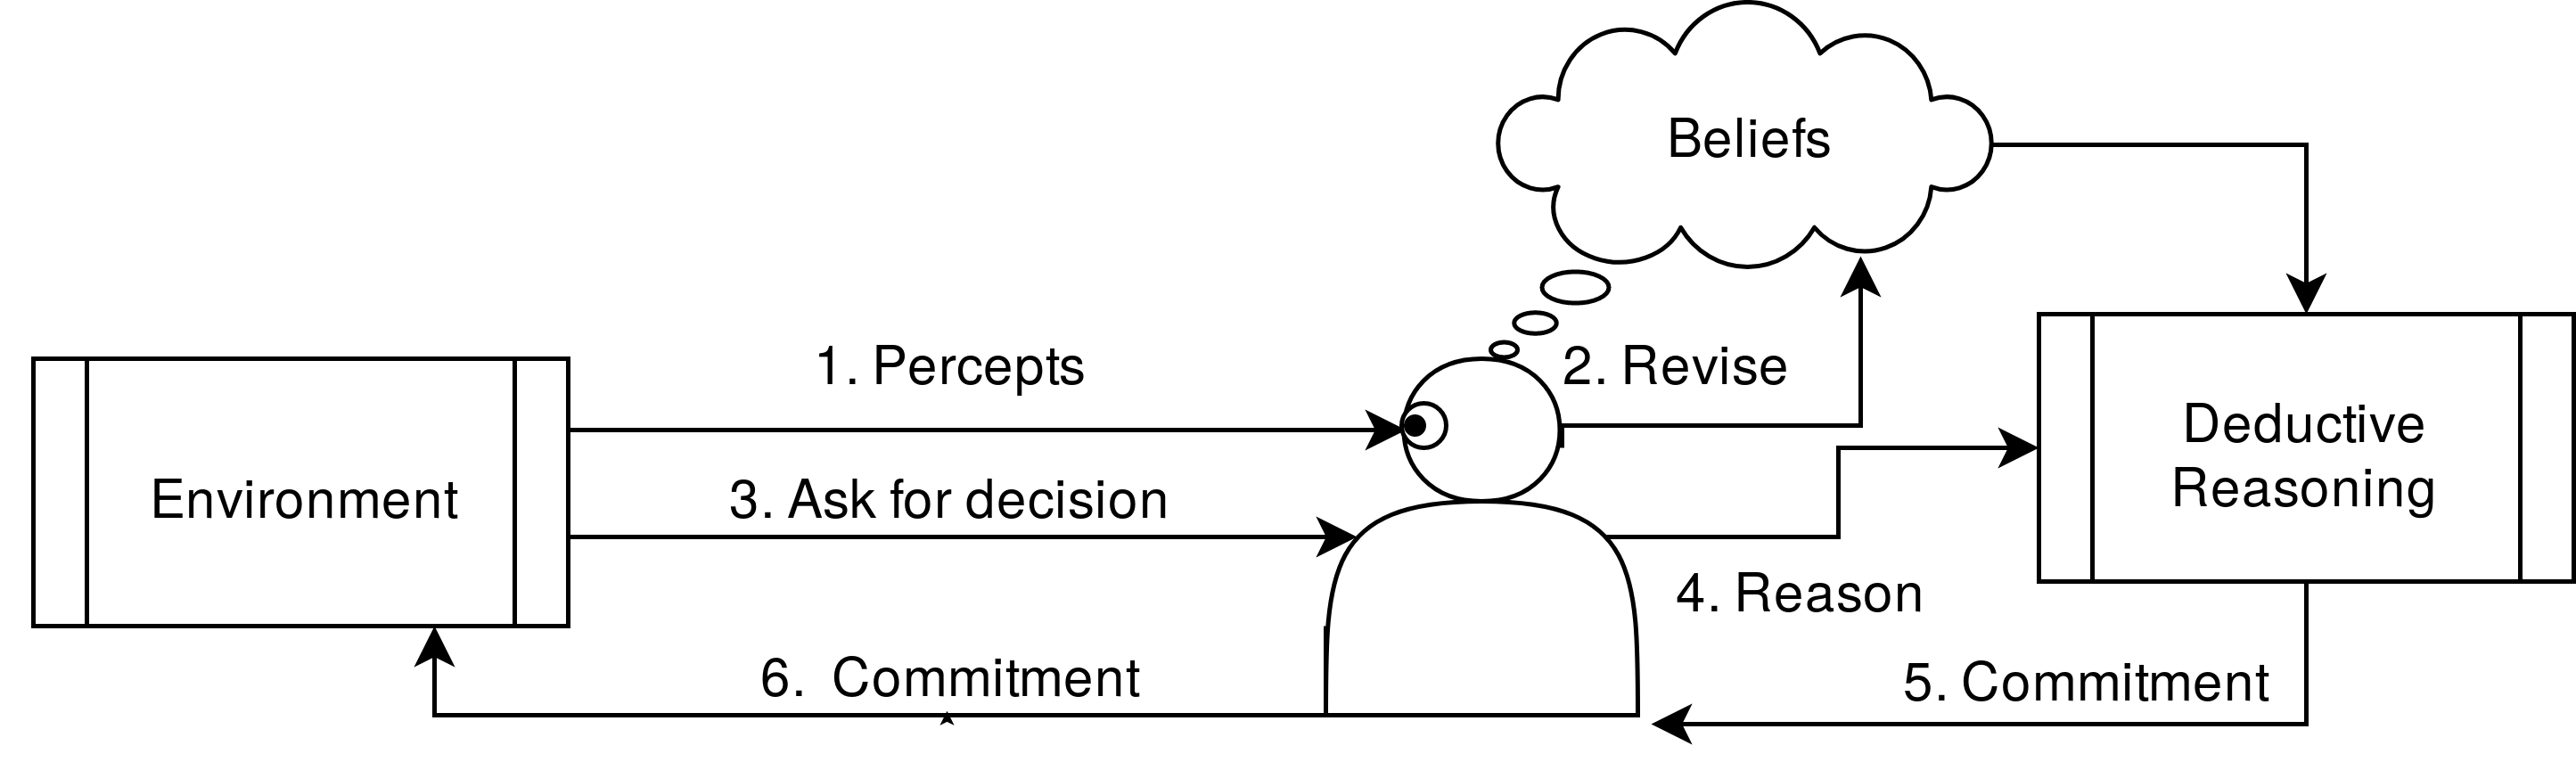
\includegraphics[width=0.5\textwidth]{PerceiveReviseDecide.png}
	\caption{Visual description of the process my agents' will follow}
	\label{fig:percept_to_action}
	\end{center}
\end{figure}
\noindent This raises the question: how do agents change their internal state based on the percepts they receive? The changing of the internal state is strategy dependent, but the overriding concept is for the agents to follow a game-theoretic approach.\\
To extend the example of the image scoring discriminator, let us say that agent1 perceives agent2 defecting against agent3. The image scoring strategy laid out by Nowak and Sigmund~\cite{evol_indirect_image} states that when a defection is perceived, the perceiving agent will lower the donor's image score in their beliefs.\\
An observation on this method: percepts cause an agent's beliefs about its environment and other agents to change at specific timepoints. This method of changing the internal state is remarkably similar to an approach to reasoning about events (similar to percepts) and time and how events change `fluents' (similar to beliefs) known as the events calculus~\cite{kowalski1989logic}.\\
Due to these remarkable similarities, the use of the event calculus seems an intuitive way to program an agent to react to percepts and query beliefs. There is a version of the event calculus known as the multi-valued fluent cached event calculus (kindly provided by my supervisor Professor Kostas Stathis) which will make querying beliefs efficient.\\
I have covered how agents will map from percepts to beliefs and then beliefs to actions. In each timepoint of an indirect reciprocity game, this mapping will be executed as part of a cycle step. The timepoints are executed in sequence, each cycle step includes in this order the processes perceive, revise (called as a consequence of perceiving) and decide. In the perceive step agents will receive percepts from the environment, passed through an API, from these percepts they will revise their beliefs. An agent will then decide on an action to take, the agent will commit to an action at the cycle step timepoint based on their beliefs.\\
The capability of an agent will be constrained at a given timepoint by way of an agent perceiving that they are the donor of a donor-recipient pair at that timepoint. The decision on which agents are donors and recipients in pairs falls to the environment. If an agent perceives they are a donor they can only cooperate or defect, but when they are not they cannot cooperate or defect. At any other point when they are not a donor they will be able to gossip or be idle.\\
In conclusion, I believe that the agent structure I have delineated matches the 4 properties Wooldridge and Jennings described~\cite{wooldridge_jennings_1995}. Autonomy has been satisfied by the way that agents have control over their beliefs, control over the actions they commit to based on these beliefs and merely choose to act based on their environment, not human action. Reactivity is satisfied by the process of receiving percepts, formulating beliefs from them, and then being able to respond to the changes in the environment by acting based on these beliefs.\\
In my system agents have 5 options as to the actions they will be able to take: idle, positive gossip, negative gossip, cooperate as a donor and defect as a donor. Both the last two properties are met by the possibility of gossip actions, and for proactivity the ability to choose between cooperating and defecting. Gossip actions are communicative actions where a gossiper communicates to another agent either positive or negative ideas about a third agent, displaying social ability. Gossip actions also show proactivity as agents can actively seek to inform other agents in a way that will affect the overall game to bring them closer to their goal.\\
An example of this is an agent whose goal it is to induce the evolution of cooperation gossiping to another agent a negative idea about an agent that it has viewed defecting, in the hope that the recipient of the gossip will then not help the defector by cooperating with them if they're a donor.

\subsection{Environment}
So far I have discussed agents in my system, but agents are useless without an environment to observe and act in. My environment will run the indirect reciprocity model I outlined in my report on indirect reciprocity. The sequence of how the environment runs is given in figure~\ref{fig:env_class} on page~\pageref{fig:env_class}.\\
The environment consists of a community that contains `generations' of players. The community simulates the indirect reciprocity model by creating and simulating a series of generations. Simulating a generation consists of running for each timepoint from start to end a cycle step. Each cycle step consists of 3 parts: perceive, decide and execute. Revision of beliefs is done as a consequence in an agent's mind of the perceive part, so is excluded from the environment's cycle step.\\
Each part of the cycle step is done for all agents at once, that is perceive sends all the percepts for a cycle step in one go, decide asks all agents to commit to a decision and then execute executes the action in the environment. Execution depends on the action if it is a gossip action or cooperate/defect action percepts are generated from this (including percepts for the selected onlookers for a cooperate/defect action) and for a cooperate action fitness is updated as per the payoff matrix in table~\ref{tab:payoffmatrix}.
\begin{framed}
	\begin{center}
		\begin{tabular}{c|c|c}
		\multirow{2}{*}{Donor Action} & \multicolumn{2}{c}{Payoffs}\\		
		& Donor & Recipient\\
		\hline
		Cooperation & -1 & 2\\
		\hline
		Defection & 0 & 0\\
		\end{tabular}
		\captionof{table}{The payoff used in my indirect reciprocity model}
		\label{tab:payoffmatrix}
	\end{center}	
\end{framed}
\noindent The execution of an action raises the question of whether my environment is or is not deterministic. Russell and Norvig specify that when deciding on this we should ignore the actions of other agents when considering the certainty of a specific actions outcome. So when we consider that a gossip action may or may not change the reputation of the agent it is about in the recipient's internal state this does not prevent the environment from being deterministic, as the internal state of an agent is controlled by that agent. Thus I adjudge that my environment is deterministic.\\
This is one of Russell and Norvig's 7 properties of a task environment, here I shall discuss further how the rest of their properties match my environment.\\
Due to the features of the indirect reciprocity model the environment is only partially observable. When I say the features of the indirect reciprocity model I am referring to actions which are only observable by a subset of the agents in a generation. An example of this is cooperate/defect actions which are only observable by the chosen onlookers and the donor-recipient pair.\\
Of course, this also highlights the environments property of being a multi-agent environment rather than a single agent environment. A more interesting question to answer on this is is the environment cooperative or competitive. This, of course, depends on whether cooperation has managed to evolve and if it is stable. But from a game-theoretic argument, even cooperative agents are competing to increase their fitness the most, the model simply encourages competition in a cooperative way.\\
The key idea behind indirect reciprocity is: if I as a donor help this recipient, agents who have seen this will, later on, cooperate with me. Due to this key idea, my environment must be sequential, that is a decision at one timepoint may have an effect on any other decision at a later timepoint.\\
Russell and Norvig state that for an environment to be discrete it must handle time and actions in a discrete way. Time in the environment I am implementing will be discrete timepoints at which each cycle step executes. Actions and percepts are also discrete as they are limited to the percepts and actions mentioned in earlier sections.\\
I have noted previously that agents all perceive, revise and decide at the same time. The consequence of this is that the environment does not change whilst the agents are deliberating over their action, thus making the environment static.\\
Finally, the rules of the environment are known to the agent. These rules include the payoff matrix for cooperate/defect actions, gossiping may or may not affect an agent depending on the recipient agents belief revision implementation and the idle action has no effect on the environment.\\
To sum up the properties of the environment I propose it is deterministic, partially observable, multi-agent, sequential, discrete, static and known. 

\subsection{Communication and API Design}
As I have mentioned previously the agents' minds will be hosted in a web service for the environment to interact with. The web service will be hosting agents' mind's and as such will need to have a creation process, this includes assigning a new mind with no previous internal state (except for any initial state which holds) and associating it with a strategy.\\
To follow the design principles of a RESTful system (REpresentational State Transfer) an individual agent is considered a resource, and multiple agents a collection. There is a specific path associated with the agent resource which includes a POST request associated with it to create a new agent. A POST request is also used to comply with RESTful design as it asks the server to create a resource. This is not a PUT request as the resource is not updated if the same request is attempted again, once an agent is created it cannot be changed, and thus the result is different (fails) if you repeat it.\\
In my system, an agent is assigned a player id, but this is not a universal identifier that distinguished it from all other agents. A player can be thought of similarly to a weak entity in a database, it is reliant on being part of a generation, which in turn is reliant on being part of a community. As such the `primary key' of a player would be the id of the community, generation and the player itself. This makes communities and generations resources as well which require universal resource indicators (endpoints). These endpoints both have POST requests which like the agents endpoint you can request the creation of a new resource too.\\
When selecting agents to start a game with a user needs to know what strategies there are to select. As such, there is an endpoint associated with the strategy resource which a GET request can be sent to in order to get a list of strategies.\\
A cycle step combines the sequence of 4 possible steps: perceive, revise, decide and execute. Perceive and decide are mandatory steps which need to be initiated by the environment. A percept is the resource linked to the perceive step, the endpoint for this needs to be able to take new percept information and create the percept resource. Creation of the percept resource involves creating an event in the event calculus, this then may or may not change values of fluents (depending on the initiates\_at and causes\_at predicates associated with the event).\\
In the decide step an agent commits to an action, the resource that is created is an action. Action has a resource endpoint which you can send a GET request to (with parameters defining which player you are asking to decide on an action and the timepoint at which they are deciding) that returns the action that the player has decided on.\\
The final resource that I have so far decided that a user of the API should is the belief resource. Agents base their decisions on beliefs about other agents and their environment, and it would be great to be able to understand why an agent has made the decision that it has. A user can make a GET request to a specific type of belief (donor, recipient, interaction and standing) with parameters depending on which type of belief the user is asking for. The GET request made will return the belief of the agent at that time, which will hopefully give a clue as to why an agent acted as they did at a specific timepoint.\\
The API is designed to follow the 6 constraints of a RESTful API: uniform interface (use of JSON throughout, resources with one endpoint, correct use of HTTP methods etc.), independent client and server, stateless communication, cacheable resource declaration and a layered system architecture (though for me the system will be one entity). Documentation can be found for the API in the repository of this project under the folder ``FullUnit\_1819\_JamesKing/AgentsService/api\_docs''. 


%------------------------------------------------

\section{Discussion and Conclusion}
In summation of my report, my agents will follow a similar architecture to model-based reflex agents. These agents will be able to make use of the event calculus to reason about how percepts change their beliefs. From this, they will be able to deductively reason as to what actions to commit to. These actions will be constrained by the idea of agent capabilities inspired by the Agent0 language.\\
The environment comprises of a number of generations, which for a certain number of cycles executes the steps perceive, decide and execute. Actions of cooperation come at a cost of 1 to the donor but a benefit of 2 to the recipient, while defections cost1 none but gives none back. Cooperate/defect actions also generate percepts for onlookers and gossip actions for recipients.

%----------------------------------------------------------------------------------------
%	REFERENCE LIST
%----------------------------------------------------------------------------------------
\bibliography{../refs.bib}{}
\bibliographystyle{plain}

%----------------------------------------------------------------------------------------

\clearpage
\begin{figure}
	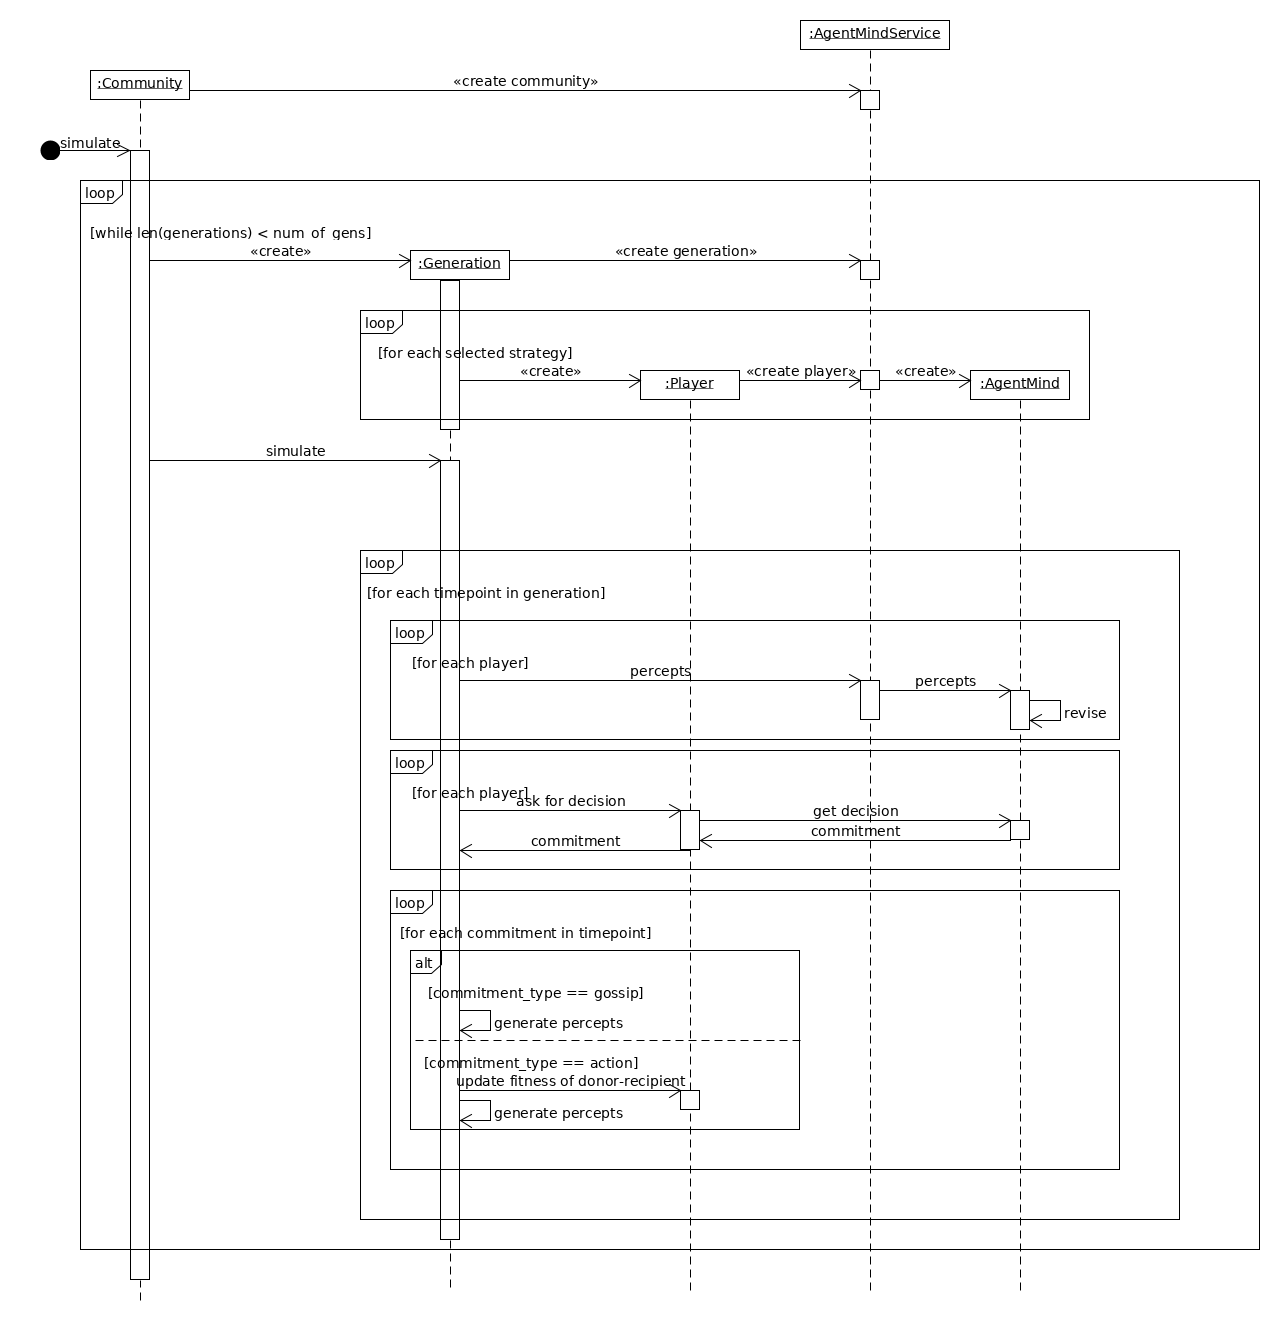
\includegraphics[width=1\textwidth]{EnvSequence.png}
	\caption{Sequence diagram for the running of the environment}
	\label{fig:env_class}
\end{figure}

\end{document}
